\documentclass[a4paper,10pt]{article}

\usepackage{graphicx}
\usepackage[utf8]{inputenc}
\usepackage[spanish]{babel}
\usepackage{hyperref}
\usepackage{listings}
\usepackage{verbatim}
\usepackage[top=2cm, bottom=1.5cm, left=2.5cm, right=1cm]{geometry}
\usepackage{pdfpages}
\usepackage{enumitem}

\begin{document}
\begin{center}

{\bf{\Huge Universidad de Buenos Aires}}\\[0.5cm]
{\bf{\Huge Facultad de ingenieria}}\\[0.3cm]

{\LARGE 66.17 - Sistemas digitales}\\[1.25cm]
{\Large }Trabajo práctico Nro. 1\\[2.3cm]
{\LARGE {\bf Contador BCD de 4 dígitos con salida a display 7 segmentos}}\\[3.5cm]
{\large Lucas Simonelli}\\[2cm]
Buenos Aires - \today
\\[5.2cm]

\end{center}

% Contacto %
{Contacto: lucasp.simonelli@gmail.com}\\[2cm]
\thispagestyle{empty}   % quita el nómero en la primer pógina



\begin{comment}
\begin{abstract}
Acá va un resumen del trabajo práctico
\end{abstract}
\end{comment}

\newpage
\tableofcontents
\newpage
\section{Objetivo}
En el presente trabajo práctico se detallará el desarrollo de un sistema digital para un contador BCD
de 4 dígitos con salida a un display de 7 segmentos, para FPGA.

\section{Diagramas en bloques}
	\subsection{Diagrama General}
	\begin{figure}[h]
		\centering
		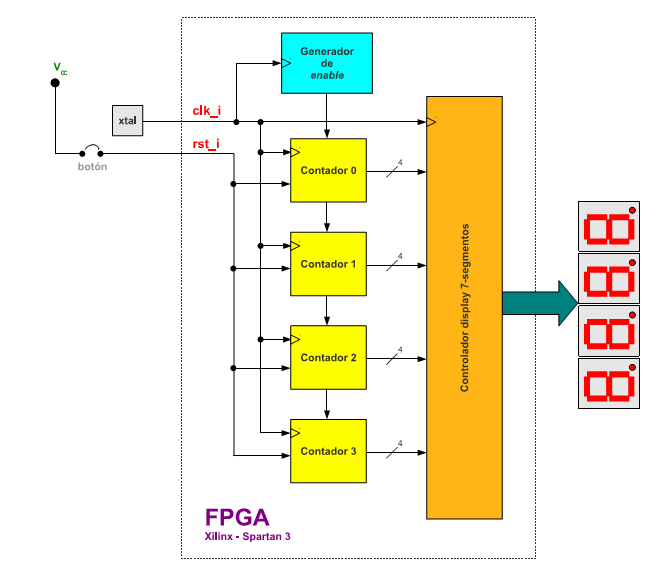
\includegraphics{img/general.png}
		\caption{Diagrama en bloques de la arquitectura propuesta por el enunciado.}
	\end{figure}

\subsubsection{Contadores BCD}
Los contadores BCD serán implementados en base a flip flops D. Se utilizará como base un contador de cuatro bits que se reseteará a 0 cuando la cuenta avance de 9 a 10.

Luego se conectarán en cascada para lograr que cuenten de 0 a 9999.

\subsubsection{Generador de enable}\label{gen}
Se implementará con un contador que devolverá un 1 cuando se llegue a 33554432 ($2^{26}$) ciclos del reloj (aprox. cada un segundo).

\subsection{Controlador display}
\begin{figure}[h]
	\centering
	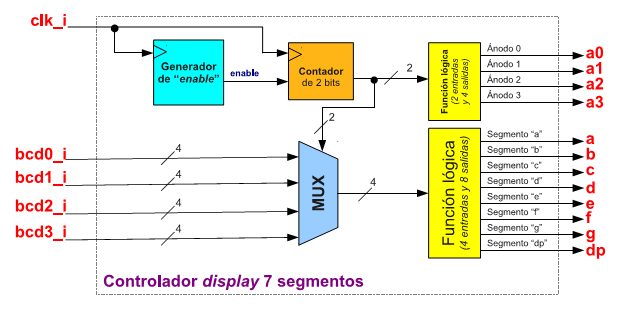
\includegraphics{img/controladorDisplay.png}
	\caption{Diagrama en bloques del controlador del display.}
\end{figure}

\subsubsection{Generador de enable}
Este generador se implementará de la misma forma que el de la sección \ref{gen}, pero cambiando el valor hasta el que se cuenta para que los dígitos roten a 1kHz.

\subsubsection{Multiplexor}
El multiplexor no se implementó por separado, sino que se realizó dentro de un process al momento de integrar los componentes.


\subsubsection{Lógica display}
\begin{figure}[h]
	\centering
	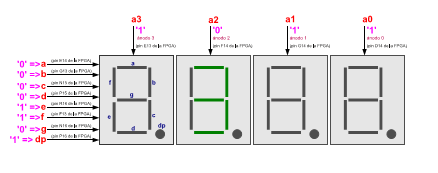
\includegraphics{img/display.png}
	\caption{Conexión de los I/O del FPGA y el display.}
\end{figure}
Se implementó una función lógica que, dada la entrada del contador correspondiente, prende los segmentos necesarios del display para que éste se muestre en la pantalla.


\section{Conclusiones}
El presente trabajo sirvió para aprender a utilizar vhdl en un nivel básico. Además, se vió como sintetizar el código y subirlo al FPGA.

\begin{comment}
\begin{thebibliography}{99}

\bibitem{INT06} Intel Technology \& Research, ``Hyper-Threading Technology,'' 2006, http://www.intel.com/technology/hyperthread/.

\bibitem{HEN00} J. L. Hennessy and D. A. Patterson, ``Computer Architecture. A Quantitative
Approach,'' 3ra Edición, Morgan Kaufmann Publishers, 2000.

\bibitem{LAR92} J. Larus and T. Ball, ``Rewriting Executable Files to Mesure Program Behavior,'' Tech. Report 1083, Univ. of Wisconsin, 1992.

\end{thebibliography}
\end{comment}
\end{document}
